\section{ 時間(とき)の翼}
\large{

\ruby{時間}{とき}の\ruby{翼}{つばさ}で\ruby{蒼}{あお}い\ruby{夕暮}{ゆうぐれ}を

\ruby{手}{て}を \ruby{繫}{つな}いで \ruby{歩}{ある}いたら

\ruby{温}{ぬく}もりが つたわる

\ruby{今}{いま}だけは\ruby{世界}{せかい}でたった\ruby{二人}{ふたり}だけ

\ruby{信}{しん}じる\ruby{気持}{きもち}

とり\ruby{戻}{もど}して\ruby{都会}{とかい}を\ruby{行}{ゆ}く\ruby{風}{かぜ}のように
\\

\parpic[r]{
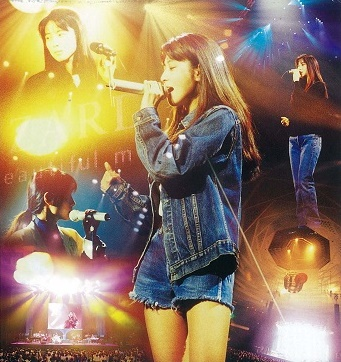
\includegraphics[width=0.4\textwidth]{P11.jpg}}
あれからぼくらは\ruby{出会}{であ}った
\\

\ruby{時間}{とき}の\ruby{翼}{つばさ}で\ruby{青}{あお}い\ruby{夕暮}{ゆうぐれ}を

\ruby{手}{て}を \ruby{繫}{つな}いで \ruby{歩}{ある}いたら

\ruby{温}{ぬく}もりが つたわる

\ruby{時間}{とき}の\ruby{翼}{つばさ}で\ruby{赤}{あか}い\ruby{夕燒}{ゆうやけ}を

くたくたになりながら

\ruby{都会}{とかい}を行く\ruby{風}{かぜ}のように

}

{ \ }
